\section{Vågutbredning på kortvåg}
\textbf{
HAREC a.\ref{HAREC.a.7.7}\label{myHAREC.a.7.7}
}

\subsection{Markvåg}

Markvågen breder ut sig längs jordytan utan kontakt med atmosfären
genom reflexion eller refraktion.

Markvågen har vertikal polarisering och en vertikal vågfront när
jordplanets ledningsförmåga är god. Vid sämre ledningsförmåga lutar
vågfronten framåt.

Markvågens räckvidd står i förhållande till den använda frekvensen,
sändareffekten och jordplanets ledningsförmåga.

Vid frekvenser under c:a 10~MHz är jordytan är en tämligen god
ledare. Markvågsutbredning utnyttjas därför mest vid låga frekvenser,
t.ex. för rundradio i lång- och mellanvågsbanden då räckvidden kan
vara i storleksordningen 1000~km. På kortvåg är markvågsräckvidden i
80 meters-bandet c:a 100 km och i 10 meters-bandet c:a 15~km.

\subsection{Rymdvåg}

Under vissa förutsättningar reflekteras radiovågorna mot joniserade
atmosfärsskikt och når åter jordytan på stort avstånd från
utsändningspunkten. Rymdvågsutbredning utnyttjas mellan platser på
jordytan med stort avstånd.

För att bäst uppnå den önskade reflexionen måste man dels välja
lämplig tidpunkt och frekvens och dels utforma antennen så att den har
sin huvudriktning i en bestämd vinkel mot det reflekterande skiktet.

Jonosfären är den del av atmosfären på c:a 50 till 350~km höjd, där
instrålningen från solen skapar fria elektroner och joner i en sådan
mängd att det bildas skikt med god elektrisk ledningsförmåga. Under
vissa villkor reflekterar dessa skikt radiovågorna, men kan under
andra villkor även absorbera dem.

\begin{figure}
  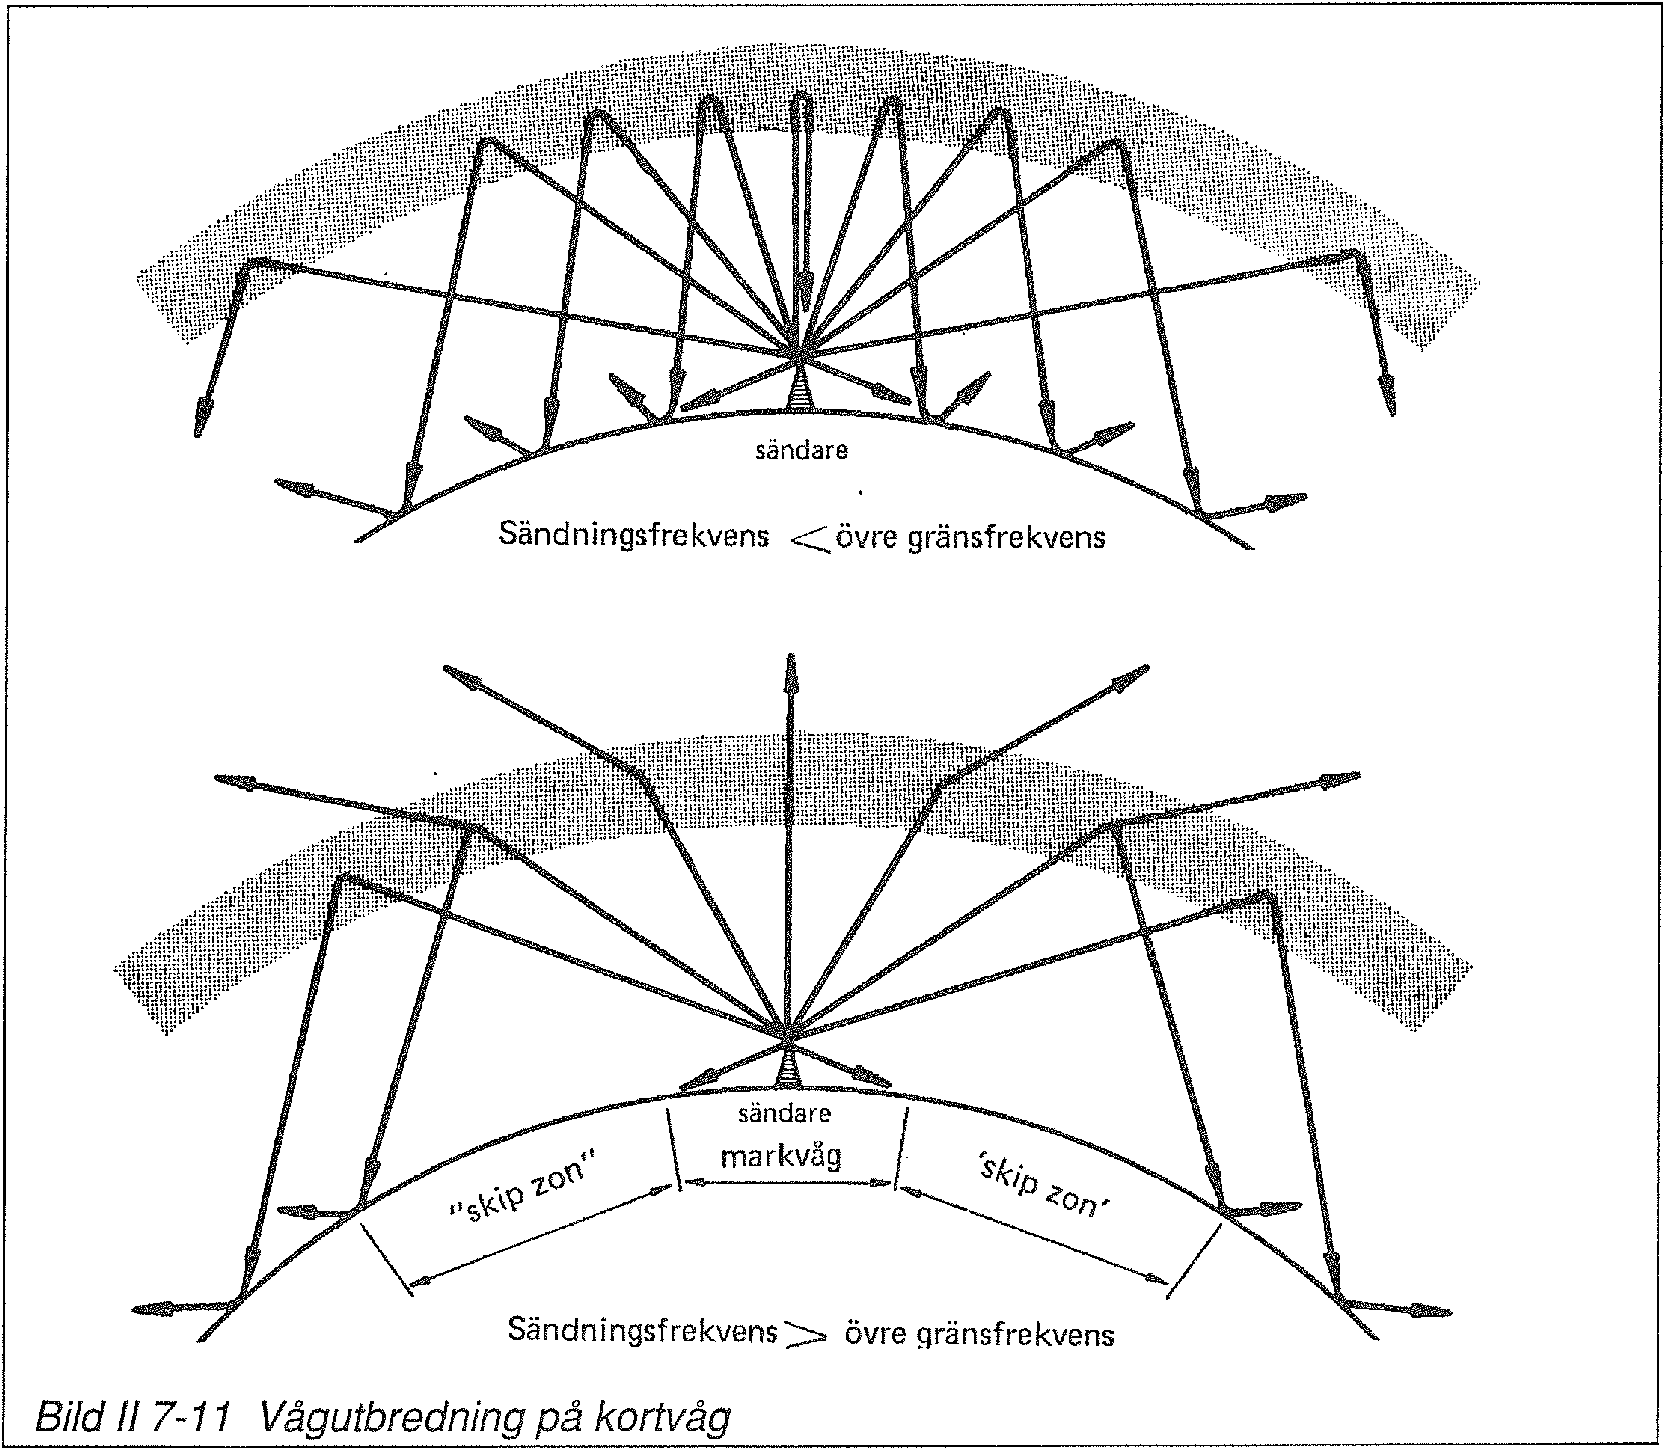
\includegraphics[width=\textwidth]{images/bild_2_7-11}
  \caption{Vågutbredning på kortvåg}
  \label{fig:bildII7-11}
\end{figure}

När vågorna från jordytan reflekterats mot de joniserade skikten, kan
de återträffa jordytan på ett avstånd av upp till 4000~km från
utsändningspunkten, beroende på frekvens och polarisering. Därefter
kan de åter reflekteras mot jordytan och upp i jonosfären
o.s.v. (flerstegshopp). Under gynnsamma förhållanden når rymdvågen
mycket långt genom växelvisa reflexioner mellan jordytan och
jonosfären.

\subsection{Död zon (skip zone) och skip-avstånd}

Rymdvågorna böjs tillbaka mot jorden när de träffar jonosfären i en
vinkel som är flackare än den s.k. kritiska vinkeln. När vågorna
träffar jonosfären med en brantare vinkel än den kritiska vinkeln sker
det ingen avböjning utan vågorna passerar genom jonosfären och rakt ut
i rymden. Beroende på den kritiska vinkeln för tillfället, kommer
därför reflekterade rymdvågor inte att höras förrän på ett visst
avstånd bort från sändaren. Detta avstånd kallas för skip-avstånd.

Men sändarens markvåg har också ett visst täckningsområde och mellan
detta och zonen där rymdvågen kan höras bildar en skymningszon - en
\emph{skip zone} eller död zon.

\subsection{Grålinjeutbredning - grayline}

Med gray line menas det smala bälte på jordytan där det för tillfället
råder gryning eller skymning.

Tidintervallet för gray line varierar med stationens latitud. Vid
ekvatorn är det \(\pm\) 5 minuter och i Skandinavien \(\pm\) c:a
\(1\frac{1}{2}\) timme omkring tidpunkten för solens uppgång
respektive nedgång.

När åtminstone en av två stationer befinner sig inom gray line kan
kortvågsförbindelse erhållas över ett mycket större avstånd än annars.

Kommunikation längs med gray line går bäst på låga frekvenser,
t.ex. på 3,5~MHz amatörband, under det tidsintervall då D-skiktet just
har börjat byggas upp (gryning) respektive nästan har brutits ned
(skymning). Då är joniseringen av D-skiktet liten och en rymdvåg som
träffar skiktet kommer då snarare att böjas av i D-skiktet än att helt
dämpas. Vågutbredningen sker då både genom refraktion i D-skiktet och
reflexion i E-skiktet.

\subsection{Fädning eller signalbortfall}
\textbf{
HAREC a.\ref{HAREC.a.7.8}\label{myHAREC.a.7.8},
 a.\ref{HAREC.a.7.9}\label{myHAREC.a.7.9}
}

Fältstyrkan på de mottagna vågorna kan variera kraftigt från ett
ögonblick till ett annat. Fenomenet kallas fädning (eng. fading,
uttalas fejding).

Sådana interferensfenomen uppstår när vågorna samtidigt vandrat flera
vägar fram till mottagarantennen, s.k. flervägsutbredning. När de
träffar mottagarantennen kan de vara tidsförskjutna sinsemellan, med
utsläckningseffekter som följd (interferensförluster).

Andra typer av fädning är när
\begin{itemize}
\item polariseringriktningen ändras p.g.a. oregelbundenheter i
  jonosfären (polariseringsförluster),
\item överföringsvägen dämpar vågorna tidsmässigt oregelbundet
  (absorbtionsförluster),
\item vågutbredningsriktningen ändras genom reflexioner mot hus,
  bergväggar etc. (reflexionsförluster, vid t.ex. mobil radiotrafik).
\end{itemize}

\subsection{Om amatörradiobanden på kortvåg}

\subsubsection{1,8 MHz (160 m):}

Bandet kallas även ``top-band''. Räckvidden är normalt relativt liten,
nattetid under vintern c:a 1200~km och i bästa fall några tusen km.
Men under solfläcksminimum kan räckvidden vara mycket större nattetid.

\subsubsection{3,5 MHz (80 m):}

Under dagtid är räckvidden ca 500 km och under kvällstid 1000--1500
km. Tidigt på morgonen under vintermånaderna, särskilt under
solfläcksminimum, är räckvidden tillräcklig för interkontinentala
förbindelser (DX = long distance). Under sommarmånaderna har bandet
hög atmosfärisk brus nivå. Döda zoner förekommer normalt inte.

\subsubsection{7 MHz (40 m):}

Detta band har större räckvidd än 80 m-bandet. Under dagtid har det en
räckvidd av 1000--2000 km. Under natten, särskilt under vintern, kan
hela världen nås. Döda zoner är 100 km under dagen och 1000 km under
natten.

\subsubsection{14 MHz (20 m):}

20 m-bandet är ett säkert DX-band för stora avstånd. Under kvällarna
ökar räckvidden på ett rymdvågshopp upp till ca 4000 km.  Särskilt
gynnsam vågutbredning erhålls vid kontakt genom en skymningszon, dvs
där den ena parten har dag och den andra har natt. Döda zoner
uppträder nästan alltid.

\subsubsection{21 MHz (15 m):}

Vågutbredningen i 15 m-bandet är bäst vid högt solfläckstal. Under
solfläcksmaximum är bandet nästan ständigt öppet för DX-förbindelser.

Under solfläcksminimum är bandet i bästa fall öppet kortare perioder
på dagtid under sommarmånaderna.

Bandet är dött nattetid. Vid reflexioner via sporadiskt E-skikt kan
avstånd av mer än 2000 km överbryggas.

\subsubsection{28 MHz (10 m):}

Bandet är lämpat för närkontakter upp till 50 km nattetid och för
DX-kontakter dagtid, dock ej dagar då E-skiktet är kraftigt joniserat
och skärmar av F-skiktet. Vågutbredningsvägen för DX är på den sida av
jorden som har dagsljus. Döda zoner på upp till 4000 km kan
uppstå. Förbindelser över stora avstånd är möjliga med låg effekt.

Under solfläcksminimum är bandet inte användbart för DX-kontakter. Då
är endast kortvariga förbindelser på avstånd upp till 2000 km möjliga
genom reflexioner via sporadiska E-skikt (short skip).

Bandet har i många fall VHF-karaktär och man kan ha kontakter via
Aurora och andra liknande utbredningsformer såsom Aurora-E och dubbelt
hopp på Auroraringen.

\subsection{10 MHz (30 m), 18 MHz (17 m) och 24 MHz (12 m):}

Vågutbredningsegenskaperna i dessa senast tillkomna amatörrradioband
är ett mellanting av respektive närmast angränsande amatörradioband.

\hilight{TODO: beskriv 30 m, 17 m och 12 m som egna band}
